\documentclass[../../eatbrain.tex]{subfile}
La pagina dedicata agli artisti segue come detto in precedenza il layout generale del sito, il \textbf{What} interno (cosa trovo nella pagina?) è ben rappresentato dal titolo in grande (Artists)  e dalla griglia contenente le immagini degli artisti; le immagini sono facilmente cliccabili e portano alla pagina dedicata all'artista. \\
Il numero degli artisti non è elevato ma nemmeno troppo basso e la mancanza di una barra di ricerca può allungare i tempi di individuazione, pur essendo disposti in ordine alfabetico. Come detto più volte questa scarsa considerazione dell'\textbf{How} è il danno più grande per l'usabilità del sito.\\
Il menù permette di raggiungere facilmente la home page in modo da esplicitare il \textbf{What} generico del sito web.
\begin{figure}[h]
	\centering
	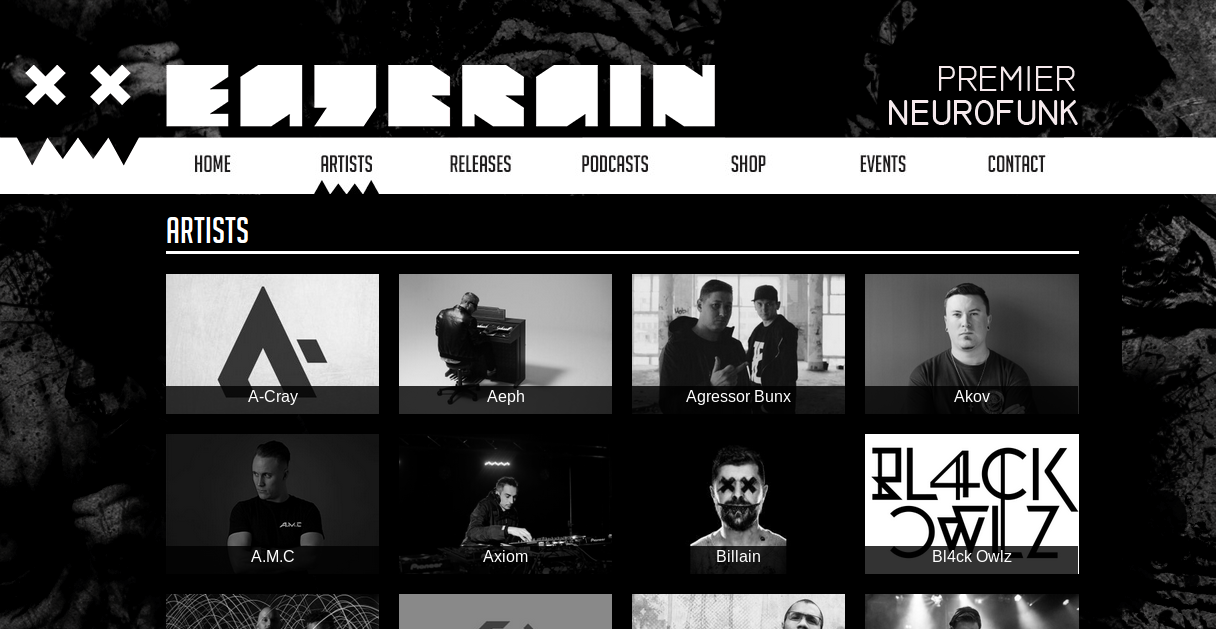
\includegraphics[width=12cm]{immagini/artists}
	\label{img-artists}
	\caption{Snapshot della pagina Artists}
\end{figure}
